\chapter{Rewards und Training}  
\label{ch:rewards_training}
In diesem Kapitel wird auf das Training eingegangen. Hierbei werden die unterschiedlichen Rewards erklärt, die genutzten Netzwerke, die Hyperparameter und die einzelnen Schritte im Training. Dazu wird auch das envScript aus Unterkapitel \ref{subsect:Airhockey Projekt} nochmal genauer beleuchtet.

\section{Rewards und Umgebungsparameter}
\label{sect:rewards_params}
Hier sollen als erstes alle implementierten Rewards vorgestellt werden, damit in den folgenden Teilen der Beschreibung des Trianings klar ist, welche Effekte sie bedingen.

\begin{itemize}
\item \underline{taskType} \\
Legt fest, welcher Spielmodus gewählt wird. Siehe dazu Abschnitt \ref{sect:spielmodi}.

\item \underline{V\_max\_puck} \\
Legt die Maximalgeschwindigkeit des Pucks fest. Einheit ist dabei nicht m/s, der Tisch ist in der Realität kleiner als in Unity. Die Ermittlung der Maximalgeschwindigkeit kann im Abschnitt \ref{sect:geschwindigkeitsmessungen} nachvollzogen werden.

\item \underline{V\_max\_robo} \\
Legt die Maximalgeschwindigkeit des Roboters fest. Messungen erfolgten analog zu denen der Maximalgeschwindigkeit des Pucks.

\item \underline{V\_max\_human} \\
Legt die Maximalgeschwindigkeit des HumanPlayer fest. Messungen erfolgten analog zu denen der Maximalgeschwindigkeit des Pucks.

\item \underline{neghumanGoalReward} \\
Dieser Reward wird gegeben, wenn der Puck in das Tor des Agenten trifft. Da es ein Gegentor ist sollte der Reward negativ gewählt werden.

\item \underline{agentGoalReward} \\
Dieser Reward wird gegeben, wenn der Puck in das Tor des HumanPlayer trifft. 

\item \underline{avoidBoundaries} \\
Dieser Reward wird gegeben, wenn der Roboter die Bande berührt. Er sollte negativ sein. 

\item \underline{avoidDirectonChanges} \\
Dieser Reward wird gegeben, wenn der Roboter die Bewegungsrichtung ändert. Er sollte negativ sein. Der Betrag wird mit dem Betrag der Bewegungsänderung im letzten Zeitschritt multpliziert. Da dieser Reward in jedem Zeitschritt gegeben werden kann sollte dieser Reward betragsmäßig sehr klein gewählt werden.

\item \underline{stayCenteredReward} \\
Dieser Reward belohnt es weder links noch rechts am Spielfeldrand zu sein. Damit kann das Verteidigungsverhalten verbessert werden. Der Reward wird zu jedem Zeitschritt gegeben und sollte deshalb sehr niedig gewählt werden. Der Reward sinkt proportional mit der Distanz vom Rand.

\item \underline{negoffCentereReward} \\
Dieser Reward ist vergleichbar mit dem stayCenteredReward. Jedoch ist dieser negativ zu wählen, denn er fällt betragsmäßig am hochsten aus, wenn der Agent an der Bande steht(links oder rechts).

\item \underline{encouragePuckMovement} \\
Dieser Reward belohnt Puckbewegungsgeschwindigkeit. Er wird zu jedem Zeitschritt gegeben und sollte deshalb klein sein. 

\item \underline{encouragePuckContact} \\
Dieser Reward belohnt Kontakte mit dem Puck. 

\item \underline{contacthalf} \\
Dieser Parameter ist kein Reward sondern eine Booleanvariable. Wird sie zu True gesetzt hat das zur Folge, das der Reward encouragePuckContact jedes mal wenn er gegeben wird halbiert wird. Damit wird verhindert, dass der Roboter alleine spielt oder den Puck einklemmt um den encouragePuckContact Reward auszunutzen.

\item \underline{playForwardReward} \\
Dieser Reward wird gegeben, wenn der Puck von hinten getroffen wird, also in die richtige Richtung geschossen wird.

\item \underline{negplaybackReward} \\
Dieser Reward wird gegeben, wenn der Puck von vorne getroffen wird, also in die falsche Richtung geschossen wird. Er sollte negativ gewählt werden.

\item \underline{negStepReward} \\
Dieser Reward wird in jedem Fall zu jedem Zeitschritt gegeben. Er soll langweiliges Zeitspiel verhindern. Dazu muss er negativ sein. 

\item \underline{negMaxStepReward} \\
Dieser Reward wird gegeben, wenn die Maximallänge einer Episode erreicht wird und das Spiel deshalb abgebrochen wird(wird nur im Training abgebrochen, nicht im Spiel).  Er sollte negativ sein.

\item \underline{behindPuckReward} \\
Dieser Reward wird zu jedem Zeitschritt, zu dem sich der Agent näher am eigenen Tor befindet als der Puck gegeben. Er sollte niedrig gewählt werden, da er in jedem Zeitschritt geholt werden kann.

\item \underline{behindPuckReward} \\
Dieser Reward ist exklusiv für das Training des Spielmoduses Defending. Er wird jedes mal gegeben, wenn ein Schuss erfolgreich verteidigt wurde.

\end{itemize}

\section{Spielmodi}
\label{sect:spielmodi}
In diesem Abschnitt werden die implementierten Spielmodi beschrieben. Mit ihrer Hilfe kann die Eignung eines Netzwerk oft schneller festgestellt werden, als mit einem ganzen Spiel, da die anderen Spielsituationen nicht so komplex sind. Ein weiterer Vorteil von einfacheren Spielszenarien ist, dass damit der Agent Stufe für Stufe traininiert werden kann.

\begin{itemize}
\item \underline{Reaching} \\
In diesem Spielmodus ist es das Ziel den Puck zu erreichen. Dazu wird der Puck zu Beginn der Episode an einem zufälligen Ort auf der Spielfeldseite des Agenten platziert. Da HumanPlayer bei diesem Szenario keine Rolle spielt wird seine Bewegung gestopt. Die Episode endet mit der Kollision von Agent und Puck oder beim Erreichen der maximalen Simulationsschritten. Damit ist dieser Modus von sehr niedriger Komplexität und auch für einen untrainierten Agenten schnell erlernbar.

\item \underline{Scoring} \\
Im Scoring Modus geht es nur ums Zielen und Tor treffen. Hier wird die Episode nicht beendet wenn der Puck getroffen wurde, sondern wenn der Puck entweder ein Tor erreicht oder die Bande trifft. Wie beim Reaching steht der HumanPlayer unbeweglich neben seinem Tor. Da mit einem diskreten Actionspace gearbeitet wird ist dieser Modus nicht viel verwendet worden. Wegen des diskreten Actionspace kann der Agent sich nicht präzise genug platzieren um zu zielen. Sollte in einem Folgeprojekt jedoch mit einem kontinuierlichen Actionspace gearbeitet werden kann dieser Modus wiede interessant werden.

\item \underline{Defending} \\
Hier hat der Agent das Ziel sein Tor zu verteidigen. Auch in diesem Modus spielt der HumanPlayer keine Rolle. Er steht dabei unbeweglich neben seinem Tor. Der Agent wird zu Beginn der Episode an eine zufällige Position auf seiner Spielfeldseite platziert. Defending ist der einzige Modus, bei dem der Puck nicht ohne Geschwindgkeit auf das Feld gesetzt wird. Der Puck wird hier von der Seite des HumanPlayer aus mit einem zufälligen Bewegungswinkel zwischen 70 und -70 auf die Seite des Agenten geschossen. Auch die Startposition wird variiert. Beendet wird die Episode wenn entweder ein Tor kassiert wurde oder der Ball abgewehrt wurde. Das ist der Fall wenn die X-Komponente der Geschwindigkeit des Pucks negativ wird, sich der Puck also auf die Hälfte des HumanPlayer zurück bewegt. In diesem Modus ist ein schneller Lernfortschritt nur mit dem defenceReward zu erwarten (bei fast allen Netzwerken).

\item \underline{FullGame} \\
FullGame ist selbsterklärend. Der Puck wird an einer zufälligen Position auf dem ganzen Spielfeld ins Spiel gebracht. Die Kontrahenten Agent und HumanPlayer werden auf ihre jeweilige Seite gesetzt und beiden ist die Bewegung im Rahmen der Parameter in envScript erlaubt. Beendet wird die Episode nur wenn ein Tor erzielt wird oder die maximale Anzahl an Simulationsschritten erreicht wird. Diesen Modus zu meistern ist das Ziel der Trainings und eine Teilaufgabe unseres Masterprojekts. Er ist zu komplex um einen untrainierten Agenten ohne das stufenweise Ändern von Rewards zu trainieren.
\end{itemize}

\begin{figure} [h]
\begin{tabular}[h]{c|c|c|c|c}
 Modus & Reaching & Scoring & Defending & FullGame \\
\hline
Puck  & Agent Seite & Agent Seite & Schuss auf Tor & Ganzes Feld \\
\hline
Agent & Agent Seite  & Agent Seite & Agent Seite & Agent Seite \\
\hline
HumanPlayer & neben Tor  & neben Tor & neben Tor & Agent Seite \\
\hline
Episodenende  & Puckkontakt & Tor, Bande & Tor verteidigt & Tor \\
 
\end{tabular}
\caption{Übersicht über die Spielmodi }
\label{modi_uebersicht}
\end{figure}

\section{Trainingsstrategie und Zwischenergebnisse}
\label{sect:trainings_strats}

In diesem Abschnitt wird das Vorgehen beim Training beschrieben und die Ergebnisse des Trainigs in der Unity Umgebung gezeigt. Um die Ergebnisse einordnen zu können werden sowohl mit Graphen der kumulativen Rewards über eine Episode als auch mit dem Ergebnissen aus Spielen von Agenten untereinander gearbeitet. Zusätzlich wird eine Einschätzung der Ästethik des Spiels betrachtet.\\

\subsection{Stufenplan}
\label{subsect:stufenplan}
Da das Spiel im FullGame Modus sehr komplex ist und viele Sachen zu beachten sind, was sich auch an der Vielzahl an sinnvollen Rewards wiederspiegelt, muss der Agent einige Vortrainings abschließen um so Eigenschaften nacheinander zu erlernen. Dazu haben wir uns einen Stufenplan der in der Abbildung \ref{training_plan} zu sehen ist, erarbeitet.

\begin{figure} [h]
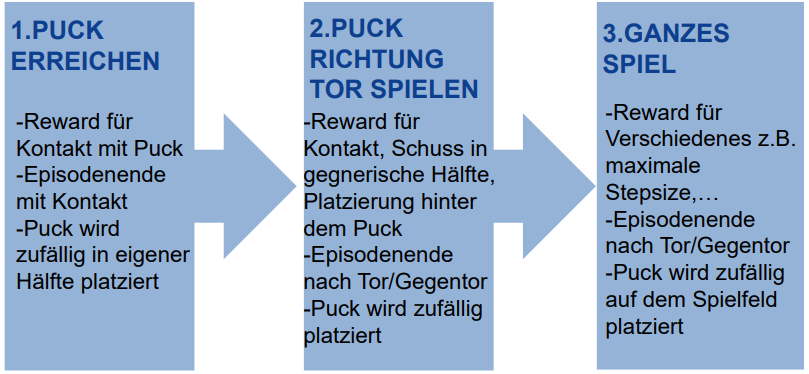
\includegraphics[scale=0.6]{images/training_strats}
\label{training_plan}
\caption{Stufenplan des Trainings}
\end{figure}

\begin{itemize}
\item \underline{1. Puck erreichen} \\
Der erste Lernschritt des Agenten ist es den Puck zu erreichen. Diese Fähigkeit kann im Reaching Modus schnell mit effektiv nur einem Reward (encouragePuckContact) erlernt werden. Ein Nachteil beim Üben im Reaching Modus ist, dass bewegte Ziele nicht vorkommen und so noch nicht trainiert werden.

\item \underline{2. Puck richtung Tor spielen} \\
Bei diesem Schritt wird auf dem vortraininierten Agenten aufgebaut. Das Ziel ist es hier den Puck in Richtung des gegnerischen Tors zu spielen. Es macht Sinn diese Fähigkeit zuerst im Reaching Modus zu üben und erst danach in den FullGame Modus zu wechseln. Dadurch ist der Anstieg an Komplexität geringer. Hier werden die Rewards playForwardReward und negplaybackReward als Hautrewards genutzt. Es hat sich jedoch gezeigt, das die Rewards encouragePuckContact und behindPuckReward hier auch nützlich sind. Dadurch wird verhindert, dass der Agent, falls er vor dem Puck erscheint, die ganze Episode abwartet um den negplaybackReward zu verhindern. Mit einem ähnlichen Satz an Rewards kann dann auch im FullGame Modus das Training fortgesetzt werden. Die Stärke des Gegners spielt dabei keine große Rolle da keine negativen Rewards für Gegentore gegebe werden.  

\item \underline{3. Ganzes Spiel} \\
Diese Stufe im Plan ist mit Abstand die zeitintensivste. Da hier das erste mal Rewards und Bestrafungen für  Tore genutzt werden ist die Wahl des Gegners nun ein sehr wichtiges Thema. Ist der Gegner zu schwach kann nicht viel gelernt werden. Ist der Gegner zu stark wird der Agent schnell passiv und versucht das Spiel auszubremsen um ein Gegentor zu verhindern. Bei diesem Schritt ist also die Balance zwischen der Anregung zum Spiel durch Rewards wie negStepReward und encouragePuckMovement und der Herrausfordernung durch den Gegner nicht einfach zu schaffen. Hinzu kommt, dass einige Reward Konstellationen zu unerwünschtem verhalten führen. Ist beispielsweise der behindPuckReward hoch, der Gegner stark in Vergleich zum Agenten und der neghumanGoalReward hoch neigt der Agent schnell dazu sich nahe ans eigene Tor zu stellen und das Ende der Episode abzuwarten. Ist der Reward avoidDirectionChanges hoch kann es passieren, dass der Roboter dazu neigt oft bis an den Rand zu fahren. Der stayCenteredReward kann hier entgegen wirken. \\ 
Dadurch das oft unvorhergesehenes schlechtes Verhalten erlernt wird ist es nach unserer Erfahrung wichtig den vorherigen Stand des Agenten zu sichern und gegebenenfalls den Vortschritt zu verwerfen weil es ehr ein Rückschritt ist. Dann kann mit einem neuen Reward- oder Parametersatz oder mit einem anderen Gegner ein weiterer Versuch vom gesicherten Stand aus probiert werden. 
\end{itemize}

\subsection{Netzwerkauswahl und Zwischenergebnisse}
\label{subsect:netzwahl_ergs}

In diesem Abschnitt sollen die Ergebnisse von zwei Netzwerken und ihren Hyperparametern verglichen werden. In diesem Stil wurden noch andere Konstellationen von Hyperparemetern verglichen. Nach Abwägung der Trainingsgeschindigkeit gegen die Komplexität wurde sich dann für die Parametersätze, die die in den Konfigurationsdateien zu finden sind, entschieden. \\
Das ML-Agents Toolkit stellt sowohl PPO als auch SAC Agenten zur Verfügung. Um nicht unnötig Ressourcen zu verschwenden macht es jedoch keine Sinn zwei unterschiedliche Agenten zu trainieren. Deshalb haben wir um uns entscheiden sowohl einen PPO als auch einen SAC Agenten jeweils das gleiche Einstiegstraining durchlaufen zu lassen. Anhand der Leistung dabei haben wir dann entschieden mit welchem Netzwerk wir weiter trainieren. \\

Das Einstiegstraining erfolgte für beide Agenten mit genau den gleichen Rewards in der gleichen Umgebung und mit den gleichen Parametern. Es beinhaltet insgesamt fünf Einzeltrainings nach denen Rewards oder Parameter angepasst wurden. 

\begin{itemize}
\item 1: Im Reaching Modus wir nur mit dem encoragePuckContact Reward das Netzwerk für 500k (500 000) Episoden trainiert. 

\item 2: Das zweite Training erfolgt immer noch im Reaching Modus, jedoch wird der encouragePuckContact Reward reduziert und der playForwardReward dazugenommen. Auch ein kleiner negStepReward wird genutzt. Das Training endet nach 1M (1 000 000) Episoden

\item 3: Dieses Training erfolgt nun im FullGame Modus. Neben den Rewards für Tore werden hier einige andere Rewards hinzu genommen um das Spielverhalten zu formen. Als Gegner wird ein anderer PPO Agent verwendet, der vorher schon etwas besser traininert wurde. Dessen Geschwindigkeit wird aber stark limitiert um das Spiel fair zu halten. Es wird so für weitere 1M Episoden trainiert.

\item 4: Nach dem letzten genannten Trainingsschritt ist aufgefallen, dass sich der Agent oft weit am Spielfeldrand befindet und so die Verteidigung vernachlässigt. Deshalb wurden für dieses Training die Rewards angepasst. Auch die Geschwindigkeit des HumanPlayer wurde erhöht um dem Agenten besser gewachsen zu sein. So wurde dann bis insgesamt 3M Episoden trainiert.

\item 5: Dieses Training unterscheidet sich nicht vom vierten. Mit den gleichen Vorraussetzungen wurde das Training bis 4M fortgesetzt
\end{itemize}

Die Ergebnisse dieser Trainings sind im folgenden Dargestellt. Im den Abbildungen sind jeweils die Graphen des PPO-Agenten und des SAC-Agenten übereinander gelegt. Der linke Graph zeigt dabei die Entwicklung des komulativen Rewards über die Anzahl der verstrichenen Trainingsepisoden, der rechte die Entwicklung der Episodenlänge. Da die Trainings aufeinander aufbauen sind in den Graphen der fortgeschrittenen Trainings die ver vorrangegangenen auch enthalten.\\
\begin{figure} [h]
\underline{1. Trainig bis 500k} 

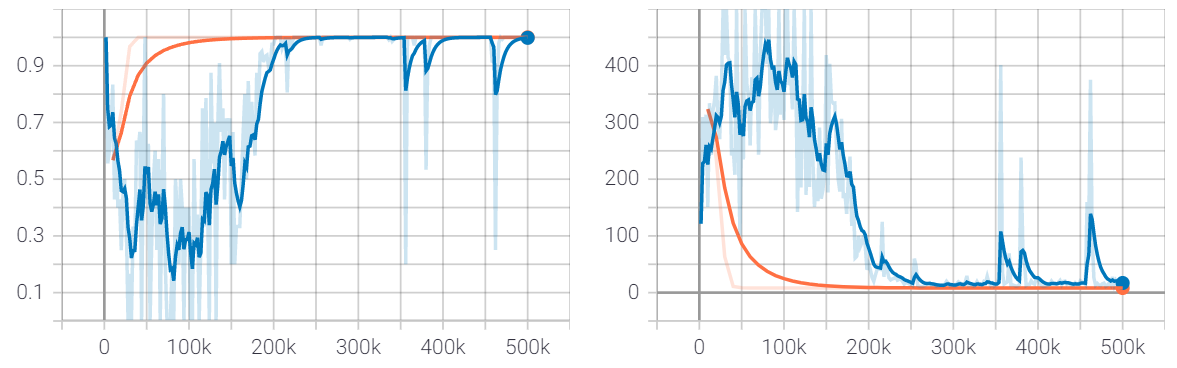
\includegraphics[width=\textwidth]{images/reaching_erg}
\label{unity_agent}
\caption{Orange: PPO-Agent, Blau: SAC-Agent}


Der maximal erreichbare kumulative Reward ist in dieser Trainingsphase 1. Am Graph ist zwar zu erkennen, dass der PPO-Agent dieses Ergebnis schneller und ohne Ausreißer erreicht, aber der SAC-Agent erreicht das Ziel auch. Beobachtet man die beiden Agenten in der Unityumgebung bei der Aufgabe sind sie vom Verhalten her praktisch nicht zu unterscheiden. Beide bewegen sich auf sehr kurzem Weg auf den Puck zu.
\end{figure}
\begin{figure} [h]
\underline{2. Trainig bis 1M} 

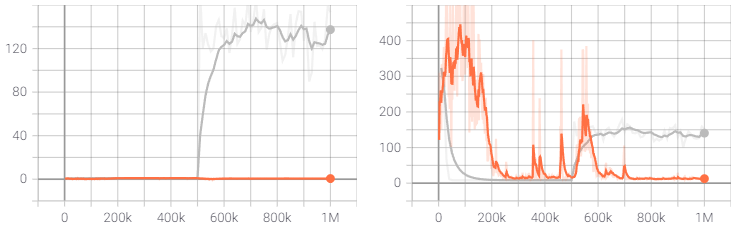
\includegraphics[width=\textwidth]{images/rea2_erg}
\label{unity_agent}
\caption{Grau: PPO-Agent, Orange: SAC-Agent}


In diesem Trainingsabschnitt hat der PPO-Agent nach Reward klar den Vorteil. Jedoch kann man an der Episodenlänge sehen, dass die Aufgabe nicht zufriedenstellent erlernt wurde. Da die Episode beim Puckkontakt beendet wird sollten sie sehr kurz ausfallen. Beim Beobachten des Spielverhalten ist dieses Verhalten auch festzustellen. Der PPO-Agent neigt dazu in der Nähe des Pucks in einen Zitterzustand überzugehen. Geht er nicht in diesen Zustand trifft er den Puck aber öfter von der richtigen Seite als von der falschen. Auch der SAC-Agent trifft den Puck öfter von der richtigen Seite als von der falschen. Er zeigt  aber die Verhaltensauffälligkeit mit dem Zittern nur äußerst selte und ist damit insgesamt besser als der PPO-Agent nach diesem Training in der zugehörigen Aufgabe.
\end{figure}
\begin{figure} [h]
\underline{3. Trainig bis 2M} 

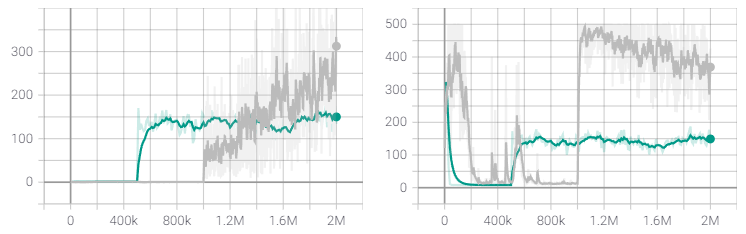
\includegraphics[width=\textwidth]{images/fullgame_erg}
\label{unity_agent}
\caption{Grün: PPO-Agent, Grau: SAC-Agent}


Der SAC-Agent hat in dieser Trainingsperiode seinen Rückstand in der Kategorie kumulativer Reward nicht nur verkürzt, sondern hat PPO sogar überholt. Die Episodenlänge hat sich dabei erhöht. Da das Trainig im FullGame Modus erfolgte und diese Agenten jetzt dafür geeignet sein sollten ist eine gute Möglichkeit sie zu vergleichen das direkte Spiel gegeineinander. Hier hat der PPO-Agent eindeutig die Nase vorne. Er schlägt den SAC-Agenten mit 10:5. Außerdem ist sein Spielverhalten deutlich besser. Währen der SAC-Agent sich oft unkontrolliert bewegt ohne den Puck zu spielen (höhere Episodenlänge) lässt sich bei seinem PPO-Kontrahenten deutlich erkennen, dass er nicht nur zielstrebig auf den Puck zufährt, sondern ihn meist auch in die richtige Richtung spielt. 
\end{figure}
\begin{figure} [h]
\underline{4. Trainig bis 3M} 

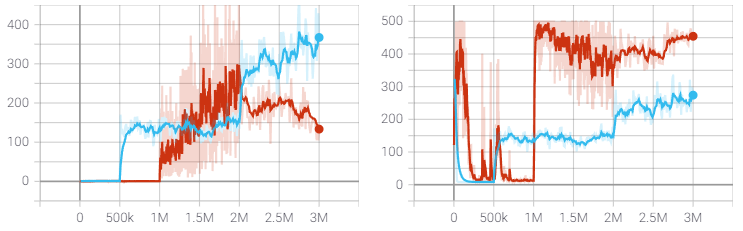
\includegraphics[width=\textwidth]{images/centered_erg}
\label{unity_agent}
\caption{Blau: PPO-Agent, Orange: SAC-Agent}


Bei diesem Training überholt der PPO-Agenten den SAC- Agenten in Sachen kumulativer Reward wieder. Auch beim Spielverhalten ist er ihm noch überleben und schlägt ihn mit 10:4. Das Verhalten des SAC-Agenten hat sich selbst nach dem Training noch nicht deutlich verbessert. Er ist immer noch sehr passiv, wenn er einen Kontakt macht ist dieser jedoch meist nicht schlecht. Insgesamt ist der SAC-Agent aber immer noch weit von einem Sieg entfernt.
\end{figure}
\begin{figure} [h]
\underline{5. Trainig bis 4M} 

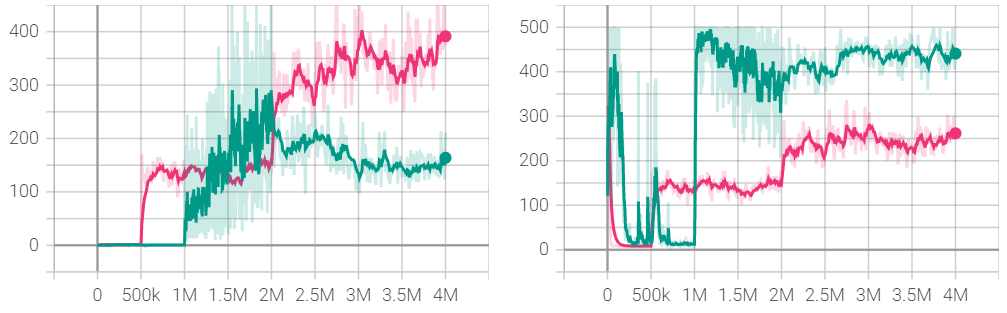
\includegraphics[width=\textwidth]{images/centered2_erg}
\label{unity_agent}
\caption{Rosa: PPO-Agent, Grün: SAC-Agent}

 
In der letzten Trainingsetappe stagnieren nicht nur die kumulativen Rewards weitgehend, sondern auch das Spielverhalten ist weitgehend unverändert. Der PPO-Agent ist dem SAC-Agenten immer noch vorraus. 
\end{figure}